\section{Auswertung}
\label{sec:Auswertung}











\begin{figure}
  \centering
  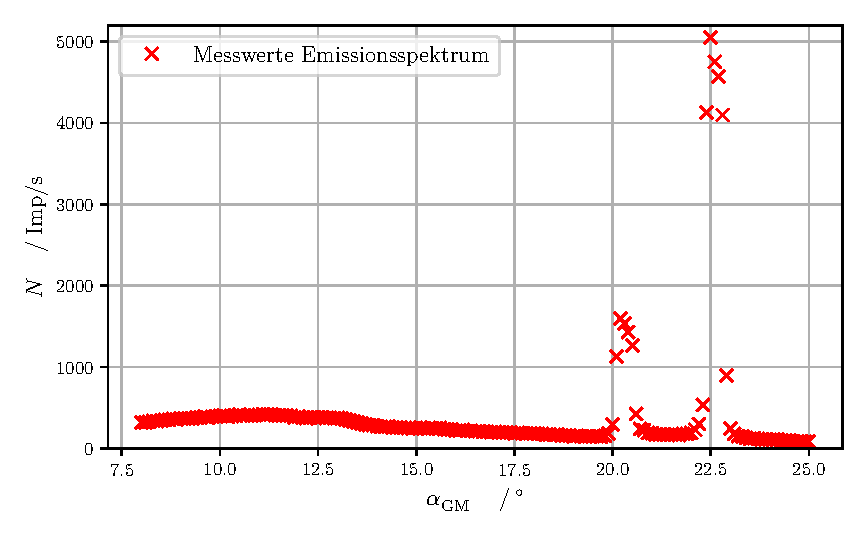
\includegraphics{build/emissionsspektrum.pdf}
  \caption{Das Emmissionsspektrum von Kupfer mit gekennzeichneten Peaks. Der erste Peak stellt $K_{\beta}$ dar, der zweite $K_{\alpha}$.}
  \label{fig:emissionssp}
\end{figure}


\begin{figure}
  \centering
  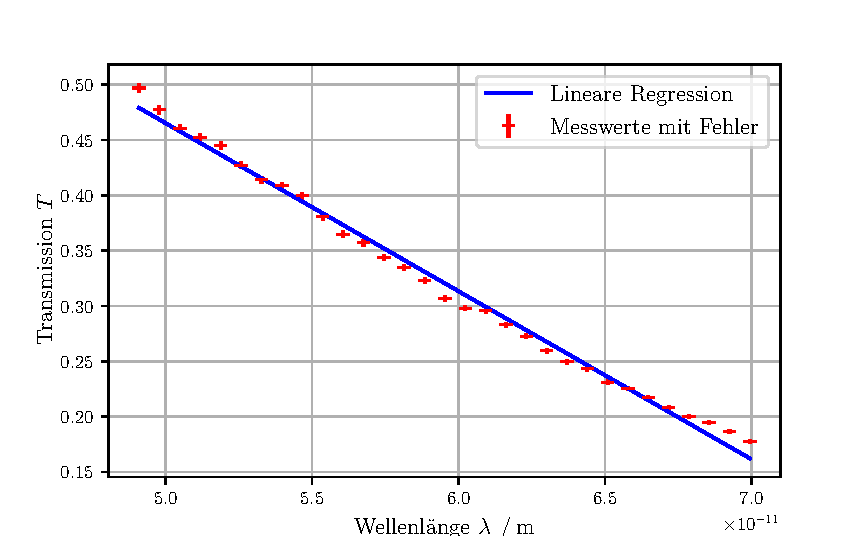
\includegraphics{build/transmission.pdf}
  \caption{Die Transmission $T$ in Abhängigkeit der Wellenlänge $\lambda$ mit linearer Ausgleichsgeraden.}
  \label{fig:transm}
\end{figure}

\begin{figure}
  \centering
  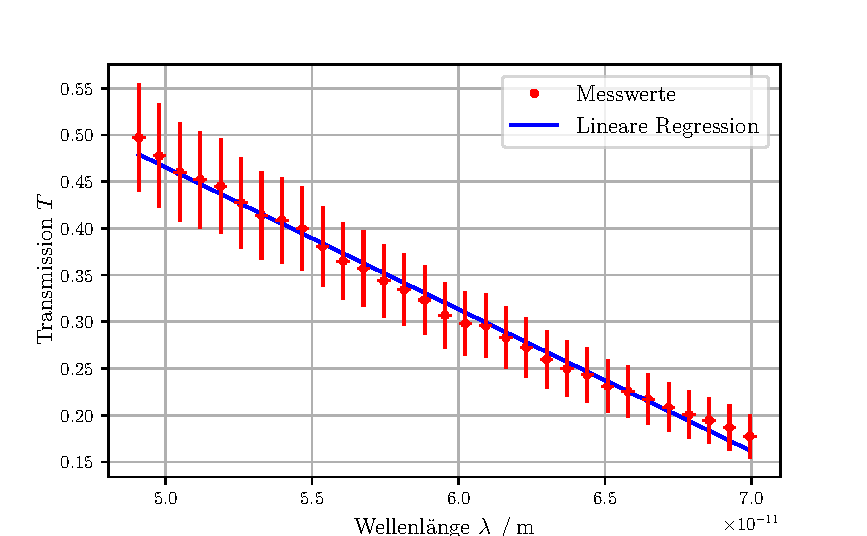
\includegraphics{build/transmission2.pdf}
  \caption{Die Transmission $T$ in Abhängigkeit der Wellenlänge $\lambda$ mit linearer Ausgleichsgeraden und Fehlerbalken.}
  \label{fig:transm2}
\end{figure}